% !TeX spellcheck = hu_HU
%----------------------------------------------------------------------------
\chapter{Alkalmazás fejlesztése és működése}
%----------------------------------------------------------------------------

\section{Backend}
A backend architekturális felépítését a korábbi fejezetben már részletesen taglaltam.  
Ebben a fejezetben az egyes rétegek és egyes funkciók megvalósításának bemutatására fektettem a hangsúlyt.
%----------------------------------------------------------------------------

\subsection{GraphQL Playground}
A legtöbb GraphQL server-hez lehetőségünk nyílik valamilyen interaktív GraphQL szerkesztő felület kiszolgálásra is.
Az alkalmazásban én a GraphQL Playground-ot használtam. Ennek a konfigurációt úgy valósítottam meg, hogy éles környezetbe ne szolgálja ki a felületet, csak fejlesztői környezet estén.
Ezt környezeti változók segítségével oldattam meg.

Azon felül, hogy interaktívan, kódkiegészítéssel szerkeszthetjük a GraphQL kódunkat kapunk egy dokumentációt is, amely tartalmazza az elérhető Query-k és Mutation-ök listáját a lehetséges paraméterekkel és a válaszok típusával együtt.
Így a használatával még kényelmesebben készíthetjük el a lekérdezéseinket, melyeknek futtatására is lehetőségünk van.

\begin{figure}[!ht]
  \centering
  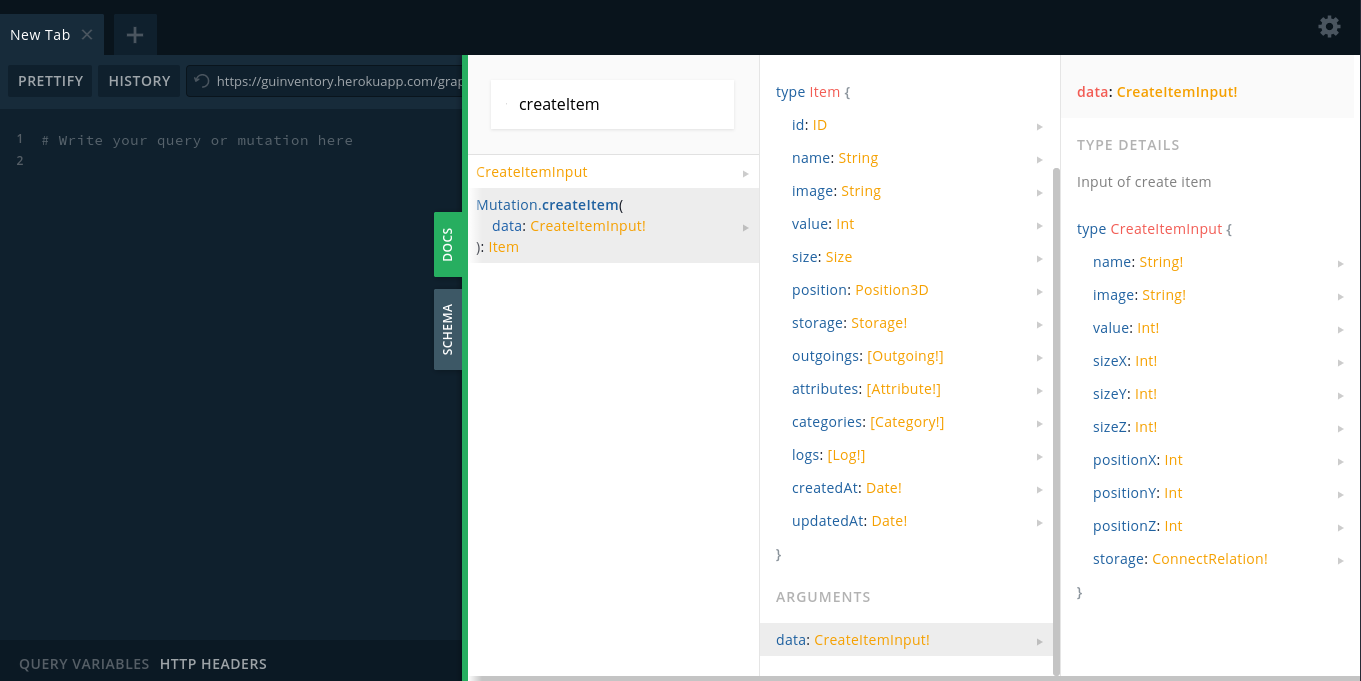
\includegraphics[width=150mm, keepaspectratio]{figures/playground_docs.png}
  \caption{GraphQL Playground Docs}
  \label{fig:playgroundDocs}
\end{figure}
%----------------------------------------------------------------------------

\subsection{Modellek és kapcsolatok}
A modell definiálásakor megadhatunk bármelyiket a sémában szereplő attribútumok közül, azonban fontos figyelni arra, hogy a típusok megegyezzenek a sémában és a modellben.
A kapcsolatokat is egyszerű mezőként kezelhetjük, beállítható továbbá az is, hogy a kapcsolat opcionális vagy kötelező illetve, hogy egy vagy több entitást tartalmazhat.
Lehetőségünk van egyedi attribútumok létrehozására is, amely az adott modell bármely attribútumából származtatható, de tetszőleges kód futtatása is megengedett, így bármilyen származtatott értéket képesek vagyunk felvenni a modelljeinkhez.

Az egyszerűség és teljesség kedvéért a példában a \lstinline|MyModel| felépítésén mutatom be egy modell definiálását.
Az \lstinline|id| és a \lstinline|name| egyszerű, az adatbázisból származó attributumok. A \lstinline|user| egy kapcsolatot reprezentál, pontosan egy darab \lstinline|User|-t tartalmaz. 
A \lstinline|custom| mező egy egyedi attributum, ami az \lstinline|id| elejére egy kettős-keresztet fűz és úgy adja vissza azt.
\begin{lstlisting}[style=ES6, caption={Példa model}]
import { objectType } from '@nexus/schema'

export const MyModel = objectType({
  name: 'MyModel',
  definition(t) {
    t.id('id')
    t.string('name')
    t.field('user', {
      type: 'User',
      nullable: false,
    }),
    t.field('custom', {
      type: 'User',
      nullable: false,
      resolve: ({id}) => `#${id}`
    })
  },
})
\end{lstlisting}
%----------------------------------------------------------------------------

\subsection{Resolver felépítése}
A Mutation-ökhöz és Query-khez tartozó resolverek minden esetben tartalmaznak egy függvényt, amely eldönti, hogy meghívásukkor milyen kódrészlet fusson le.
Ezen felül a használatukhoz szükségünk van metainformációkra is, ezért tartalmaz egy visszatérési típust, hogy pontosan tudjuk milyen típussal térhet vissza, valamint opcionálisan tartalmaz egy argumentum listát, ami meghatározza, hogy milyen paraméterek szükségesek és milyen paraméterek opcionálisak a meghívásához.
A paraméter lista meghatározza a paraméterek típusát is.

Az alábbi példában egy egyszerű létrehozásra láthatunk egy lehetséges implementációt.
A kódrészletben látható, hogy az argumentum lista helyett használhatunk külön definiált bemenetet is, így növelve a kód olvashatóságát.
A resolve függvényben elvégezhetjük a szükséges adatbázis műveletet és meghívhatunk külső függvényeket is.
A csatolt kódban az eszköz létrehozáson felül meghívjunk egy függvényt, amely elkészíti az eseményhez tartozó napló bejegyzést, valamint küldünk egy jelzést az elem létrehozásához.
Ezekre a jelzésekre a GraphQL Playground vagy bármilyen kliens segítségével feliratkozhatunk egy egyszerű websocket kapcsolattal.

\begin{lstlisting}[style=ES6, caption={Eszköz létrehozás resolver}]
t.field('createItem', {
  type: 'Item',
  args: { data: CreateItemInput.asArg({ required: true }) },
  resolve: async (_, { data: { storage, ...rest } }, context: Context) => {
    const item = await context.prisma.item.create({
      data: {
        storage: { connect: storage },
        ...rest,
      },
    })
    await log({
      type: 'CREATE',
      entityId: item.id,
      entityName: 'Item',
      newValues: { storage, ...rest },
      context,
    })
    await publishItemEvent('itemCreated', item, context)
    return item
  },
})
\end{lstlisting}
%----------------------------------------------------------------------------

\subsection{Autentikáció és autorizáció}
Az autentikáció és autorizáció ellenőrzésére a GraphQL Shield-et használtam. 
Ennek segítségével egy egyszerű JavaScript object-tel megadható, hogy egyes Query-k és Mutation-ök esetén, milyen validáció fusson le.
Lehetőséget biztosít egy úgynevezett fallback rule beállítására is, amely minden külön nem specifikált kérésnél fut le.
Ezzel valósítottam meg a bejelentkezett felhasználó validálását.

\begin{lstlisting}[style=ES6, caption={GraphQL Shield}]
export const shield = GQLShield(
   {
     Query: {
       warehouses: isGlobalAdmin,
       logs: isGlobalAdmin,
     },
     Mutation: {
       login: allow,
       register: allow,
     },
   },
   {
     allowExternalErrors: true,
     fallbackRule: fallbackRule,
   },
)
\end{lstlisting}

Az authentikációt JSON Web Token segítségével végzem. 
Sikeres bejelentkezés esetén a backend egy tokent küld a frontend részére, melyet a böngészőbe elmentve a későbbiekben minden kéréshez csatolni tudunk.

\begin{figure}[!ht]
  \centering
  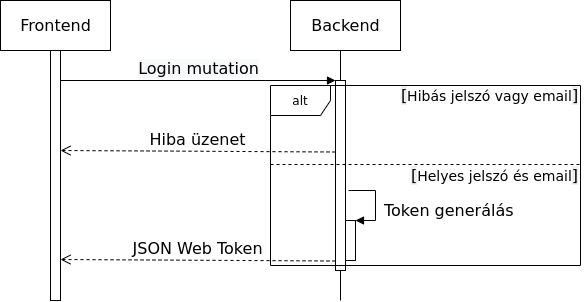
\includegraphics[width=150mm, keepaspectratio]{figures/login.png}
  \caption{JWT Bejelentkezés}
  \label{fig:JWT}
\end{figure}
%----------------------------------------------------------------------------

\subsection{Képek kezelése}
Az alkalmazáson belül lehetőségünk van kép feltöltésre a raktárba vett eszközökről.
A képek tárolására a Google Cloud Storage szolgáltatását használtam. 
A képeket feltöltés előtt base64-es formátumra kódolom át és elküldöm a backend részére.
A backend végzi a kép feltöltését a Google Cloud Storage rendszerébe és eltárolja a kép URL címét az adatbázisba a megfelelő eszköz attribútumai között.
%----------------------------------------------------------------------------

\section{Frontend}

%----------------------------------------------------------------------------

\subsection{Kódgenerálás}
%----------------------------------------------------------------------------

Ahogy az korábban már többször is szóba került az Apollo-nak hála remek kódgenerálási lehetőségeink vannak.
Alább egy példa keretein belül szeretném bemutatni ennek használatát

A GraphQL Mutation-t paraméterekkel ellátva szükséges megírnunk, hogy a kód generátor tudja lehetséges paramétereket. 
\begin{lstlisting}[style=ES6, caption={GraphQL Shield}]
mutation Login($email: String!, $password: String!) {
  login(data: { email: $email, password: $password }) {
    token
  }
}
\end{lstlisting}

A generálást futtatva azonnal használhatjuk az elkészült hook-okat (jelen esetben a useLoginMutation hook-ot).

A hálózati kapcsolat kezelésén felül megkapjuk annak az állapotát is, így tudjuk a felhasználói felület kinézetét a kérés állapotához kötni.
Például töltés esetén egy töltő képernyőt megjeleníteni, vagy a hibákat kezelni.

\begin{lstlisting}[style=ES6, caption={Bejelentkezés kódrészlet}]
const { register, handleSubmit, errors } = useForm<Inputs>()
const [login, { loading }] = useLoginMutation()
const toast = useToast()
const { setAuthToken } = useAuthToken()

const onSubmit = async (inputData) => {
  try {
    const {
      data: {
        login: { token },
      },
    } = await login({
      variables: inputData,
    })
    setAuthToken(token)
    window.location.href = '/'
  } catch (error) {
    toast({
      title: error.message,
      status: 'error',
      duration: 3000,
      isClosable: true,
    })
  }
}
\end{lstlisting}
%----------------------------------------------------------------------------

\subsection{Útvonalválasztás}
NextJS használatával alapértelmezetten fájl alapú útvonalválasztást használhatunk.
Ez azt jelenti, hogy az oldal URL-jét a fájl neve és a szülő mappák nevei határozzák meg.
Lehetőségünk van paraméterek használatára is, ezt szögletes zárójelek közé írt névvel jelezhetjük.
A paramétert ezzel a névvel fogjuk elérni a kódbázison belül is.
Ilyen paraméterrel jelzett adhatunk bármelyik szinten lévő fájlnak, de akár mappának is.


\dirtree{%
	.1 /.
	.2 auth
	.3 login.tsx
	.3 register.tsx
	.2 index.tsx
	.2 warehouse
	.3 [warehouse_id]
	.4 edit.tsx
	.4 edit_roles.tsx
	.4 index.tsx
	.4 storage
	.5 [storage_id]
	.6 edit.tsx
	.6 index.tsx
	.6 item
	.7 [item_id]
	.8 cost
	.9 [cost_id]
	.10 edit.tsx
	.8 edit.tsx
	.8 index.tsx
	.7 index.tsx
	.5 new.tsx
	.3 new.tsx
%----------------------------------------------------------------------------

\subsection{Validáció}
A felhasználótól érkező adatok minden esetben validálva vannak, ehhez a yup csomagot használtam.
A yup segítségével definiálhatunk egy sémát, amelyre a bemenetnek illeszkedni kell. 
Hiba esetén egy hibaüzenetet is generál az egyes mezőkhöz, így visszacsatolást adhatunk a felhasználónak, hogy melyik adat hibás és miért.
Amennyiben szeretnék eltérni az alapértelmezett beállításoktól, a hibaüzeneteket szövegezését a séma definiálással együtt adhatjuk meg.

\begin{lstlisting}[style=ES6, caption={Esköz validációs séma}]
import * as yup from 'yup'

export const itemSchema = yup.object().shape({
  name: yup.string().required(),
  image: yup.string().required(),
  value: yup.number().required().typeError('Must be a number'),
  positionX: yup.number().required().typeError('Must be a number'),
  positionY: yup.number().required().typeError('Must be a number'),
  positionZ: yup.number().required().typeError('Must be a number'),
  sizeX: yup.number().required().typeError('Must be a number'),
  sizeY: yup.number().required().typeError('Must be a number'),
  sizeZ: yup.number().required().typeError('Must be a number'),
})
\end{lstlisting}

A formok elküldését egy React hook-kal valósítottam meg.
A hook visszaadja a hibákat és lehetőséget biztosít a form újra-beállítására is.
Minden beviteli mezőt regisztrálni kell a form hook-ba, így biztosítva azok elérését.

\begin{lstlisting}[style=ES6, caption={Regisztrációnál használt form hook}]
const { register, handleSubmit, reset, errors } = useForm<Inputs>({
  resolver: yupResolver(itemSchema),
})
\end{lstlisting}

A hibákat egy JavaScript objektumban kapjuk meg, melynek a kulcsa minden esetben az adott beviteli mező neve.

\begin{lstlisting}[style=ES6, caption={Form}]
<form onSubmit={handleSubmit(onSubmit)}>
  <FormControl mb={4} isInvalid={!!errors.name}>
    <FormLabel htmlFor="name">Name</FormLabel>
    <Input name="name" type="text" ref={register} />
    <FormErrorMessage>{errors.name?.message}</FormErrorMessage>
  </FormControl>
  ...
</form>
\end{lstlisting}

%----------------------------------------------------------------------------

\subsection{Felhasználói felület}
A felhasználói felületet a ChakraUI könyvtár segítségével készítettem el.
A Chakra hála az összes általános komponens egy szép és minden lehetséges állapotra felkészített változatban rendelkezésemre állt.

\begin{figure}[!ht]
  \centering
  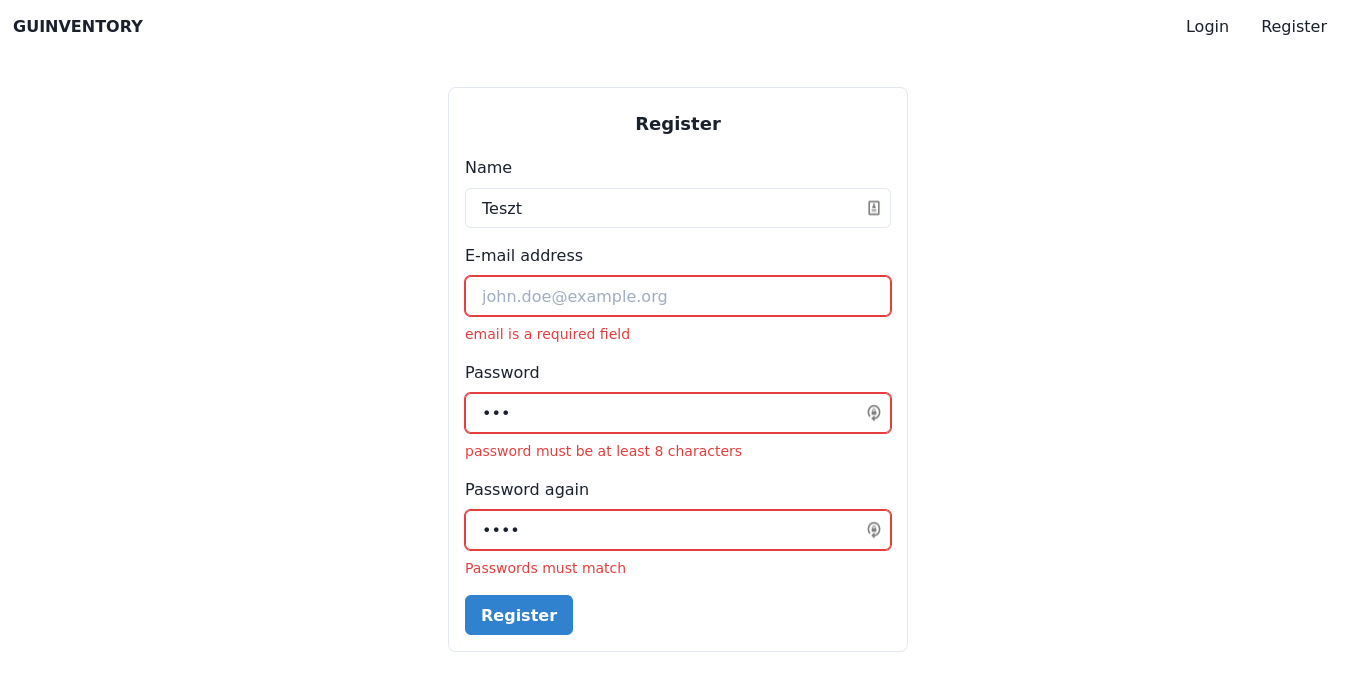
\includegraphics[width=150mm, keepaspectratio]{figures/reg.png}
  \caption{Regisztrációs oldal}
  \label{fig:reg}
\end{figure}

A regisztrációs oldalon (\refstruc{fig:reg}) láthatjuk a beviteli mezőket különböző állapotban.
Hibásan kitöltött mező esetén felhasználó azonnali visszajelzést kap a hibás adatról.
Javítás után a hibaüzenet automatikusan eltűnik, amint megfelelő formátumú adatot gépelt be a felhasználó.

\begin{figure}[!ht]
  \centering
  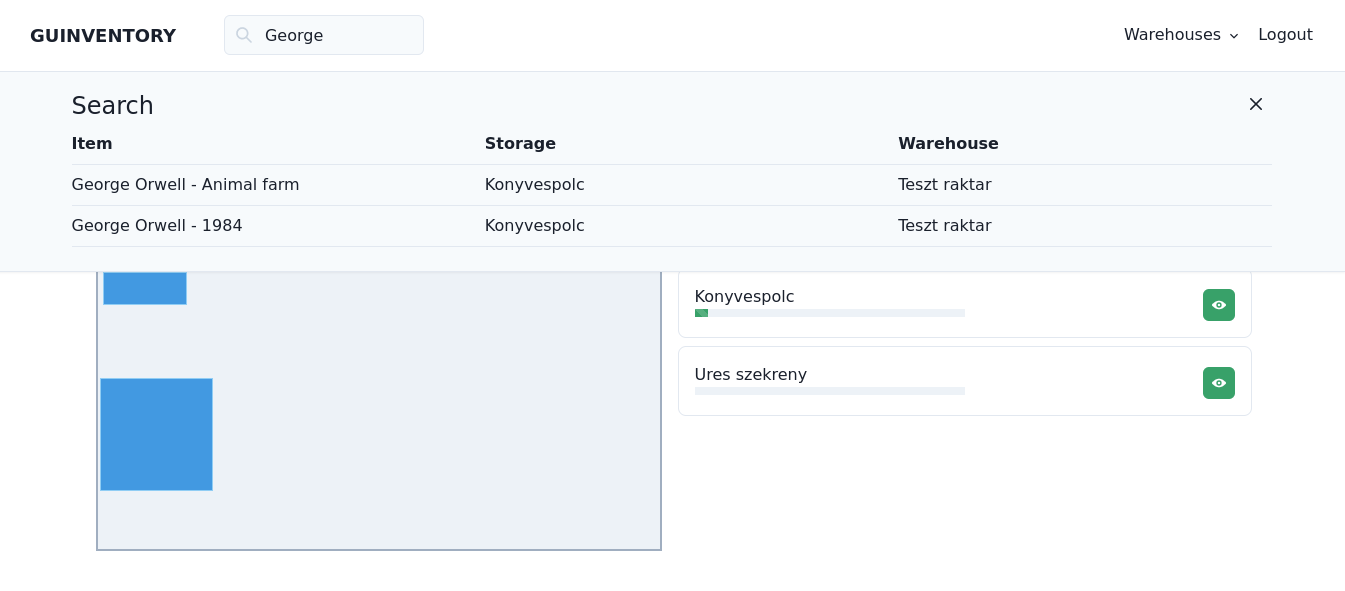
\includegraphics[width=150mm, keepaspectratio]{figures/search.png}
  \caption{Keresés}
  \label{fig:search}
\end{figure}

A keresés eredményét egy 3 oszlopos táblázatban (\refstruc{fig:search}) jelenítjük meg.
A három oszlop segítségével egyértelműen meghatározható a keresett eszköz holléte.
Lehetőségünk van a keresett eszköz raktárára, tárolójára vagy magára az eszközre navigálnunk.

A tároló nézetén (\refstruc{fig:storage}) a kurzort valamelyik eszköz fölé mozgatva megjelenítjük annak a nevét és ezen felül kiemeljük a listában is, hogy elősegítsük az azonosítást.
Természetesen ez a kiemelés másik irányba is megvalósul, tehát ha a listában választjuk ki, akkor a térképes nézeten fogjuk kiemelten látni az éppen kiválasztott eszközt.

\begin{figure}[!ht]
  \centering
  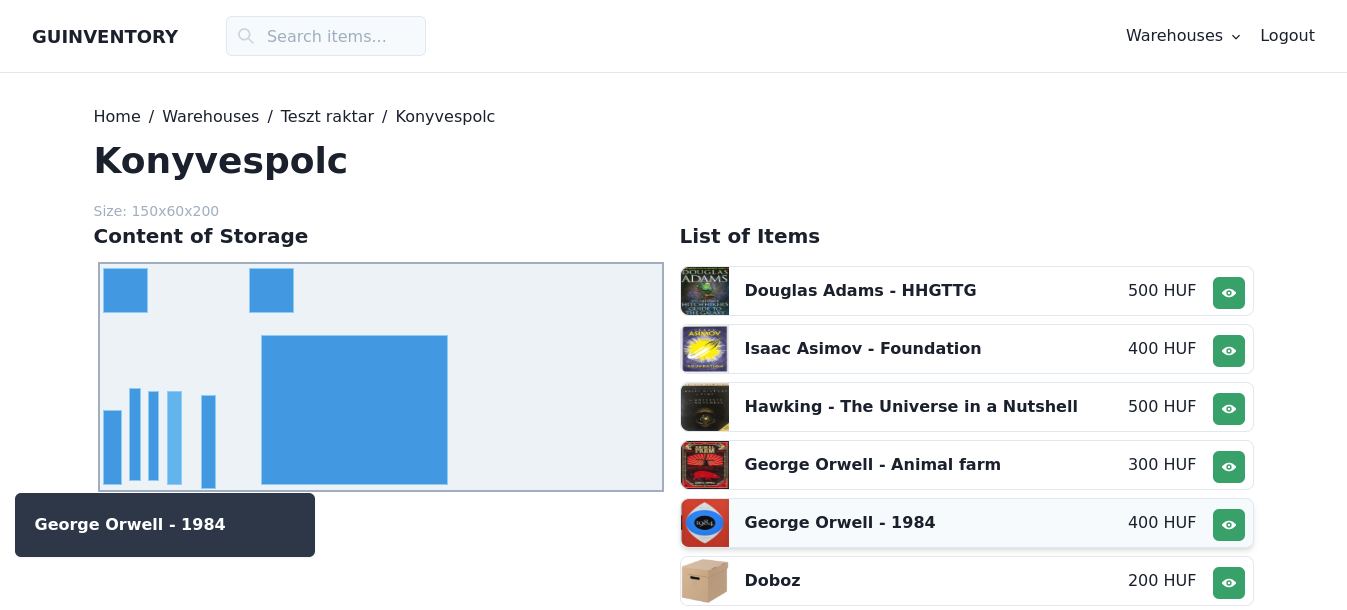
\includegraphics[width=150mm, keepaspectratio]{figures/storage.png}
  \caption{Tároló oldal}
  \label{fig:storage}
\end{figure}

A raktár nézetén belül a tárolóhoz hasonlóan kiemeléssel jelezzük az éppen kijelölt tárolót.
A tárolókról extra információként megjelenítjük az adott tároló becsült kihasználását.
A becslés a tároló méretéből és a benne tárolt eszközök méretéből számolt értékét.
Természetesen pontosan kihasználtságot nem tudunk adni, mivel a tárolókat általában nem lehet 100\%-osan kitölteni.

\begin{figure}[!ht]
  \centering
  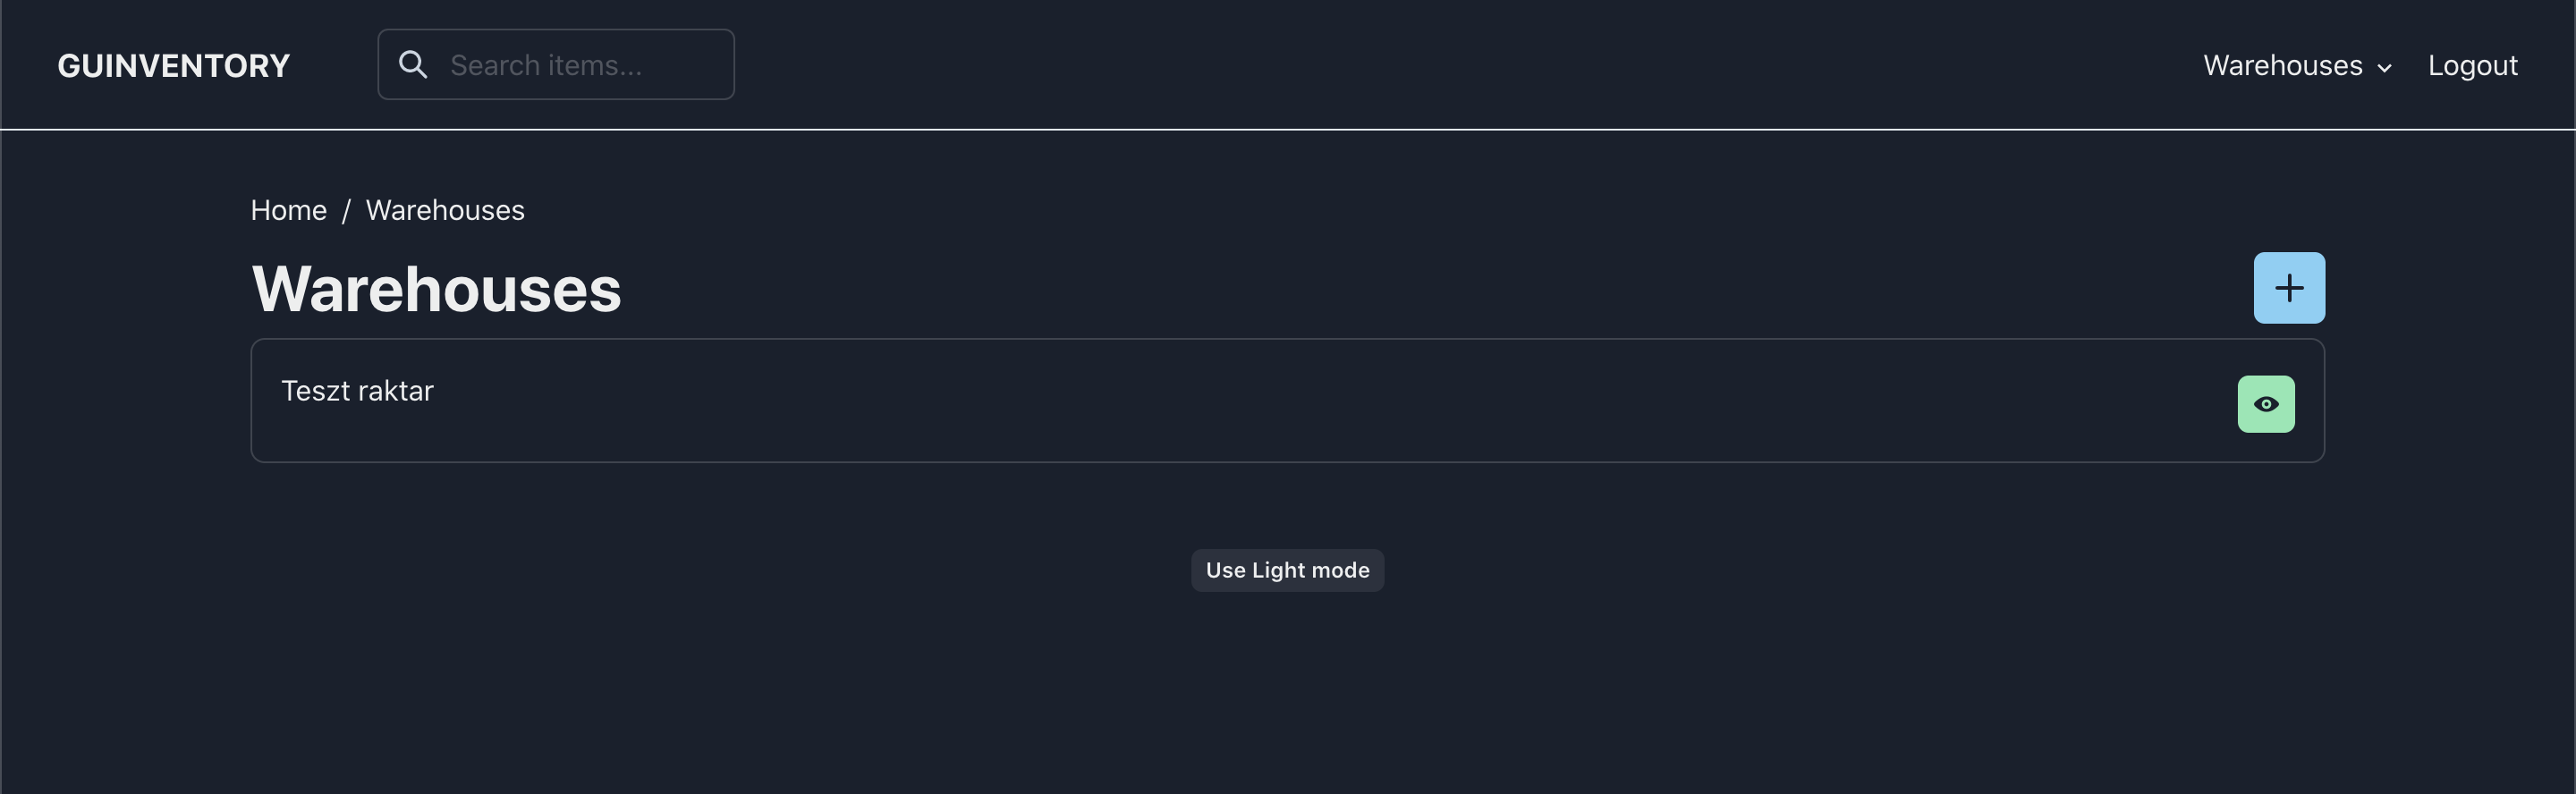
\includegraphics[width=150mm, keepaspectratio]{figures/dark_mode.png}
  \caption{Sötét téma}
  \label{fig:darkMode}
\end{figure}
A ChakraUI segítségével egyszerűen megvalósítható a sötét és világos téma is az alkalmazáshoz, valamint az e kettő közötti váltás is.
Ez jelen esetben egy sötétkék árnyalatú designt (\refstruc{fig:darkMode}) eredményezett. 
A bejelentkezett felhasználó az oldal alján található gomb segítségével válthat témát.
A választott témát az alkalmazás automatikusan elmenti a böngésző helyi tárolójába, így az oldal újbóli meglátogatásakor már a korábban kiválasztott téma lesz érvényes.


%----------------------------------------------------------------------------
